
Outline:

- Motivace
- Co je responzivní design
- Responzivní design v LaTeXu
  - přizpůsobení velikosti fontu velikosti zobrazení
  - typografická stupnice
  - media queries
    - změny počtu znaků na řádek
    - okraje pomocí newgeometry
- Automatizovaná sazba
  - luvlna
  - luawidowcontrol
    - sází odstavec na zkoušku, pokud detekuje 
  - linebreaker

 
\begin{frame}
  \frametitle{Porovnání různých metod k omezení parchantů}
  \begin{center}
  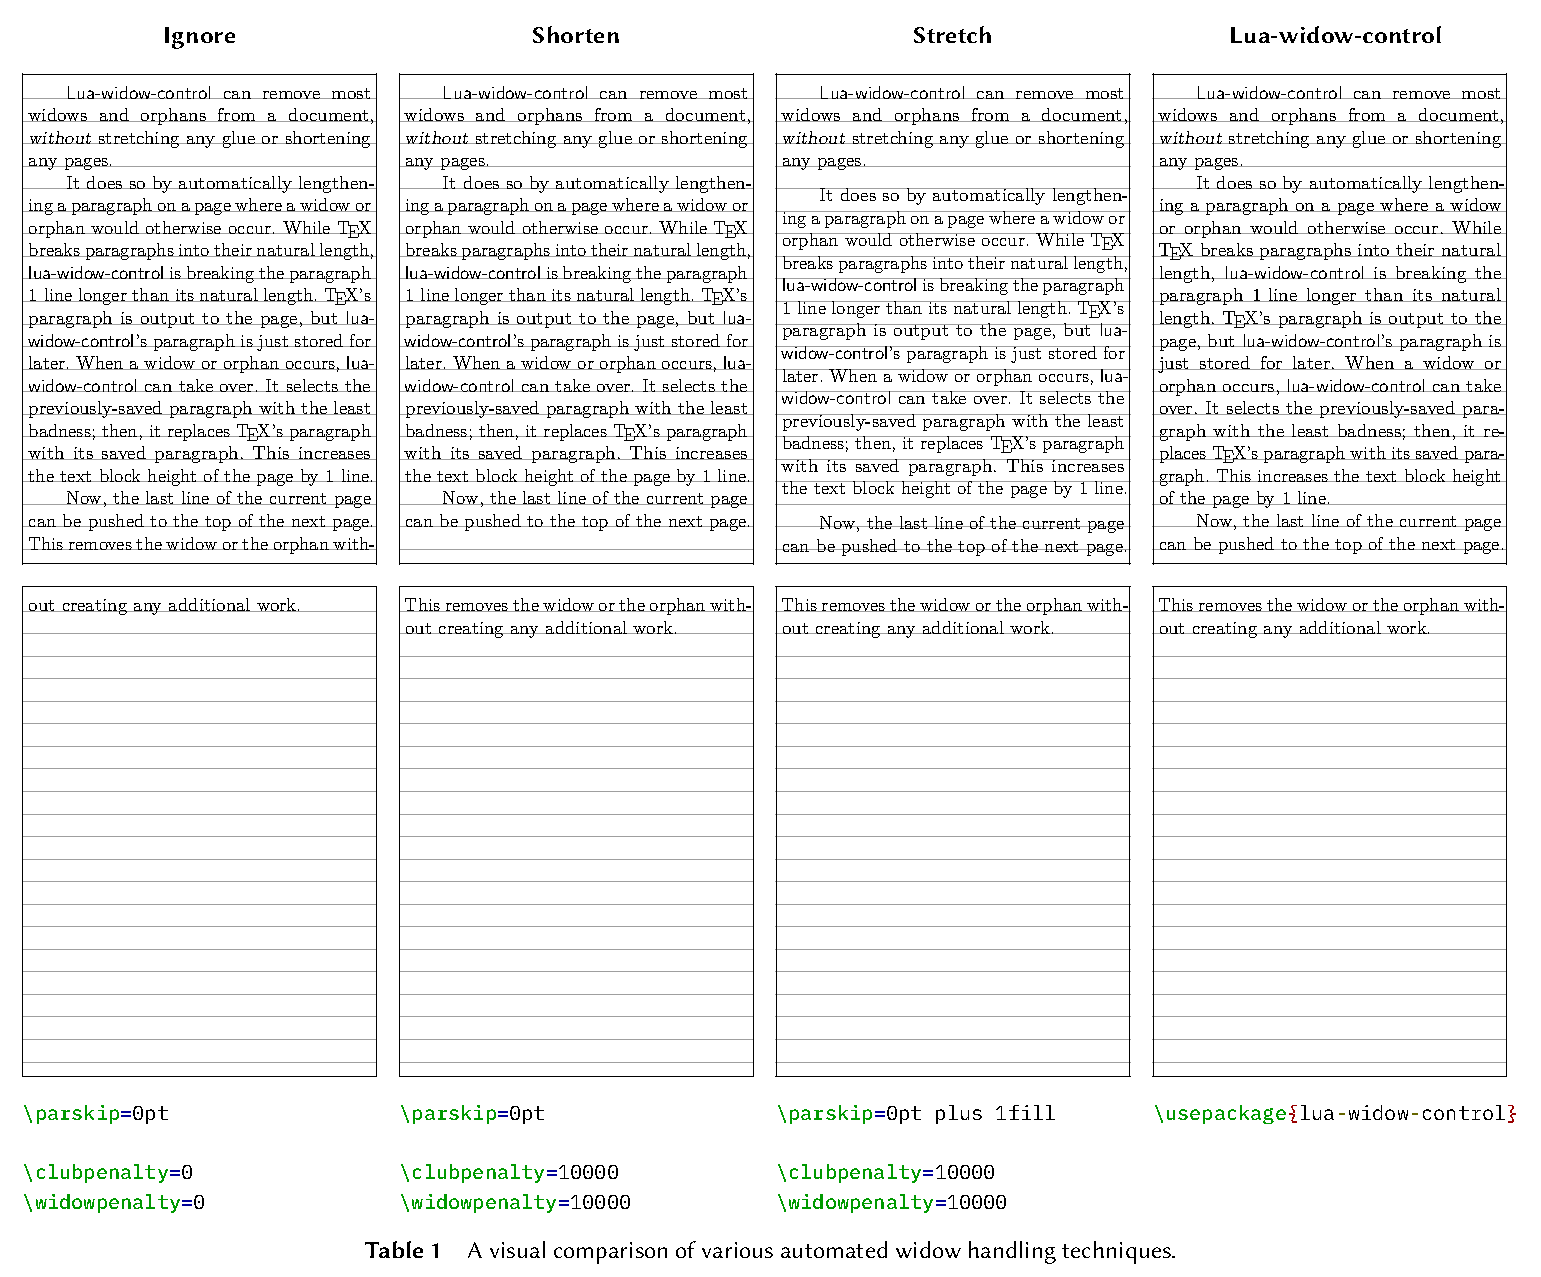
\includegraphics[height=.95\textheight]{img/lua-widow.pdf}
  \end{center}
  % \myfig[height=0.8\textheight]{img/lua-widow.pdf}{}
\end{frame}



\begin{frame}
  \frametitle{How are hooks configured}
  \begin{itemize}
    \item hooks are configured using the \texttt{\textbackslash Configure} command
    \item either in the output format file (html4.4ht, html5.4ht, ooffice.4ht)
    \item or in the private configuration file
    \item the output format can define options that are passed to the \texttt{tex4ht.sty} package
    % \item soubory výstupního formátu mohou definovat volby, které ovlivňují konfiguraci háčků
    % \item po vložení háčků se nahrají jejich konfigurace v závislosti na výstupním formátu
    % \item další konfigurace je možné vložit do .cfg souboru, který se načítá pomocí volby \texttt{-c} příkazu \texttt{make4ht}

\end{itemize}
\end{frame}

\begin{frame}[fragile]
  \frametitle{\texttt{tex4ht.sty} package options}
    they are used by the output format for a conditional configuration

  \begin{itemize}
    \item they can be passed on the command line
    \item or in a private configuration file 
  \end{itemize}
  \begin{priklad}
\begin{verbatim}
$ make4ht filename.tex "mathml,mathjax"
\end{verbatim}
\end{priklad}
\end{frame}
